
\section{Introduction}
Precipitation plays a major role in many natural and societal systems, but direct observations of precipitation are not available for all areas. Remote sensing platforms such as satellites provide estimates of temperature via measurements of elecromagnetic radiation. Temperature and precipitation are closely related due to the physical mechanisms which govern precipitation. Furthermore there is strong spatial structure in both temperature and precipitation, so the ability to describe spatial dependence is highly desirable for models of precipitation. We consider modelling precipitation given temperature on a regular grid of pixels, where the values of each pixel corresponds to average amounts over a fixed time window. Graphical models provide a natural approach for taking into account the spatial dependencies inherent in patterns of precipitation.

\section{Precipitation dataset}
We will use PERSIAN-CCS data set which consists of temperature data as well as features related to a particular cloud patch in which a pixel is part. Each pixel, which represents a small geographic area, has 1 temperature feature and 12 features related to its cloud patch. There is also a target $y$ value for that pixel obtained via radar data. The region of interest is the western United States and the temperal resolution under consideration is the finest available, 30 minutes. The following web link provides a more detailed description of the data set. 

\begin{lstlisting}
http://chrs.web.uci.edu/research/satellite_precipitation/activities01.html
\end{lstlisting}



\section{Model: Exponential Family with Conditional Random Field}

\subsection{Introduction}

Conditional Random Fields are discriminative models for the conditional distribution of labels $y$ given observations $x$. For our purposes it will be defined over a graph structure as follows:
\[
p(y|x) = \frac{1}{Z(x)} \prod_i{\psi(y_i,x)} \prod_{c}{\psi(y_c,x)}
\]
Here, $Z(x)$ is the partition function that normalizes the distribution, $\psi(y_i,x)$ is the potential function for the states of node $i$ given the input $x$, and $\psi(y_c,x)$ is the potential function for the states of nodes in clique $c$ given the input $x$. \\
\\
We will take a 2-D image and make each pixel a separate node in our graph. Our graph will be a 4-connected grid so two pixels will be connected via an edge if they are immediate neighbors horizontally or vertically. \\
\\
Our input consists of features for each node and edge, denoted by $x_i$ and $w_c$ respectively. The edge features for clique $c$ are used to obtain a conditional distribution of values for the nodes connected by $c$ and the node features for node $i$ are used to obtain a distribution of values for only node $i$. Our equation now becomes as follows:
\[
p(y|x) = \frac{1}{Z(x)} \prod_i{\psi(y_i,x_i)} \prod_{c}{\psi(y_c,w_c)}
\]
For our purposes, $\psi$ will be an exponential family. We will learn two matrices $\theta$ and $\phi$. The matrix $\theta$ will be multiplied by the node features to determine the log potentials for each value of node $i$. The matrix $\phi$ will be multiplied by the edge features to determine the log potentials for each pair of values for the nodes $i$ and $j$ connected by an edge in our graph. The model is now as follows:
\[
p(y|x) = \frac{1}{Z(x)} \prod_i{exp(\theta x_i)} \prod_{ij}{exp(\phi w_{ij})}
\]
Our goal will be to find $\theta$ and $\phi$ matrices that minimize a loss function given our training data. In our results, the loss function is defined as the clique logistic loss (Domke 2013)
\[
L = - \sum_c {log \, \mu(y_c; \theta, \phi, x_i, x_j, w_c)}
\]
Here $\mu$ signifies the accuracy of the clique marginal. \\
\\
The CRF library used employed a method it referred to as Truncated Fitting for learning. In summary, this method involved performing N iterations ($N=5$ for our implementation) of inference and then calculating the loss function regardless of whether or not convergence has occurred. The gradient of the loss function is then computed and this is used to update the model parameters. Finally, N iterations of inference are done in reverse order.  \\
\\
The inference method employed was Tree-Reweighted Belief Propagation. This method replaces the marginal polytope with a super-set before computing the message passing updates. Approximations are done to ensure there is a tractable upper bound on the log partition function (Domke 2013). 

\subsection{Feature Setup}

The features associated with each node consist of the temperature as well as the 12 cloud patch features from the CCS data. There is one additional feature that is a constant. The cloud patch features are zero when there is no cloud. Additionally, we added an additional feature that is 1 for a cloud pixel and 0 for a non-cloud pixel to be sure that $\theta$ focuses only on precipitation versus no precipitation pixels for the cloud ones. There are thus a total of 15 features for each node. \\
\\
Since the first node feature is temperature, we will define the following:
\[
\Delta x_{ij} = |x_{i1} - x_{j1}|
\]
The edge features used were inspired by computer vision labeling problems and consisted of the temperature differences between neighbors parameterized as a set of thresholds. More formally, let $T = \{ T_0 , T_1, ..., T_M \}$ be a set of thresholds. Given the set $T$ and a value $s$, we will define a function that returns a vector of which thresholds it passes as follows
\[
h(s,T) = ( \delta (s \geq T_0), \delta (s \geq T_1), ..., \delta (s \geq T_M))
\]
In our case, we will use $T_i = \frac{i}{20}$ for $i$ from $0$ to $M$ and $M=10$. For a given edge between neighbors $i$ and $j$, the edge feature vector will be as follows
\[
w_{ij} = h( \Delta x_{ij}, T)
\] 

\subsection{Results}

Our training data consisted of temperature and precipitation information from September 2011. There were readings every half hour thus there were a total of 1440 maps. Due to the large size of the data set, I used a random subset of 160 maps for training. We then used maps from September 2012 as our test set. \\
\\
Here is an example of one of the September 2012 maps. Results for the other maps were quite similar. These are the target precipitation labels. 
\begin{figure}[h]
\centering
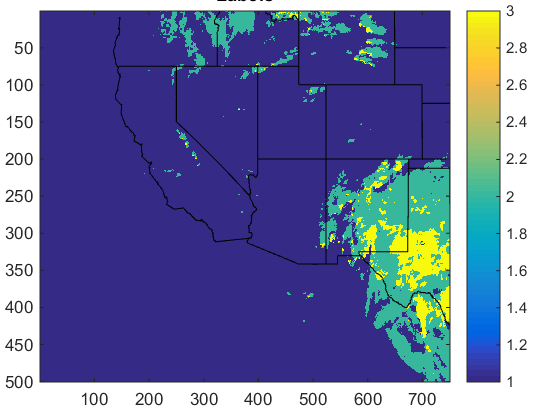
\includegraphics[width=3in]{./zackWriteUp/time1196_labelMap.png}
\caption{Probability of Rainfall}
\end{figure}
Here are the marginal probabilities of rainfall across the image.
\begin{figure}[h]
\centering
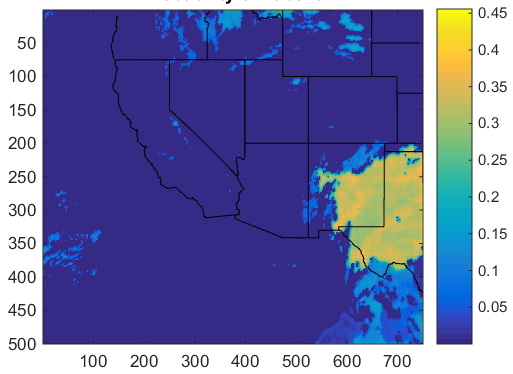
\includegraphics[width=3in]{./zackWriteUp/time1196_probPrecip.png}
\caption{Probability of Rainfall}
\end{figure}
Here are some of the statistics \\
**TABLE OF PROBABILITY INFORMATION FOR THE MAP**\\
Naively, these were our prediction stats:\\
**INSERT THEM**\\
Because the marginal probabilities rarely exceeded $0.5$ we needed a smaller threshold for our predictor if we ever wanted to predict precipitation with this model. After doing ROC analysis, as can be observed in figure **REFERENCE**, we picked a threshold of **INSERT WHAT IT WAS** and these were our prediction accuracies: **INSERT STATS**. 


\subsection{Conclusion}

There are problems with this model. There is low probability of precipitation even in the pixels where it occurred. This could be due to the fact that we have highly imbalanced classes. There could also be problems with our edge features as they are inspired by a different application. \\
\\
One potential fix is a rethinking of the edge features. The current edge features do not correlate well **INSERT STATISTIC SHOWING THIS** with the target pairs of states for the nodes. We need to find edge features that show some correlation with pairs of states for neighboring nodes. One idea is to use the temperature difference but only for the cloud pixels. Another idea is to use one of the cloud patch features. We could also use a combination of mean temperature between pixels and difference between them. 


